% This file was converted to LaTeX by Writer2LaTeX ver. 1.9.9
% see http://writer2latex.sourceforge.net for more info
\documentclass{article}
\usepackage{calc,amsmath,amssymb,amsfonts}
\usepackage[LGR,T1]{fontenc}
\usepackage[greek,english]{babel}
\usepackage[style=numeric,backend=biber]{biblatex}
\usepackage{array,supertabular,hhline}
\usepackage[pdftex]{graphicx}
\usepackage{hyperref}
\hypersetup{
    colorlinks=true,
    linkcolor=blue,
    filecolor=magenta,      
    urlcolor=cyan,
    pdftitle={Overleaf Example},
    pdfpagemode=FullScreen,
    }
\setlength\tabcolsep{1mm}
\renewcommand\arraystretch{1.3}
\title{ClassClock Admin Interface Training Manual}
\author{Adrian Edwards}
\date{2023-08-06}
\begin{document}

\begin{titlepage}
    
	\begin{FlushRight}
		\vspace*{1cm}
			
		\Huge
		\textbf{Thesis Title}
			
		\vspace{0.5cm}
		\LARGE
		Thesis Subtitle
			
		\vspace{1.5cm}
			
		\textbf{Author Name}
	\end{FlushRight}

	\normalsize
	\textbf{Revision Information:}\\
	\begin{FlushLeft}
		% \tablefirsthead{}
		% \tablehead{}
		% \tabletail{}
		% \tablelasttail{}
		\begin{tabular}{m{3.5em}m{3.35316in}m{1.4233599in}m{0.8615598in}}
		{Revision} &
		{Description of changes} &
		{Changed by} &
		{Date}\\

		{0.1} &
		{Initial Version} &
		{Adrian Edwards} &
		{11/26/2022}\\

		{0.2} &
		{Added headings for individual tasks and added arrows to the “click and drag” image for
		clarity. Add section for setting up an account in the admin panel} &
		{Adrian Edwards} &
		{1/3/2023}\\

		{0.3} &
		{Move intro, background, and human process description up to the top. Use an automatic table of
		contents for the task listing so it stays up to date. Move revision information to title page} &
		{Adrian Edwards} &
		{8/5/2023}\\
	\end{tabular}
	\end{FlushLeft}
		
	\vfill
	\begin{center}
        
		{This work (including all images contained within) is licensed under the Creative Commons Attribution-ShareAlike 4.0
		International License. To view a copy of this license, visit \href{http://creativecommons.org/licenses/by-sa/4.0/}{http://creativecommons.org/licenses/by-sa/4.0/}.}



		
\includegraphics[width=1.439in,height=0.5043in]{Mini20Manual-img001.png}
            
    \end{center}
\end{titlepage}
\clearpage




\newpage
\setcounter{tocdepth}{3}
\tableofcontents

\bigskip


\bigskip


\bigskip


\bigskip

\clearpage
\bigskip

\section{Software Description}
\subsection{Introduction}
{ClassClock is a tool that is designed to simplify the day-to-day lives of students and staff in a K12 educational
setting by providing a quick and easy countdown to indicate when class ends based on the schedule for the day.}

\subsection{Background}
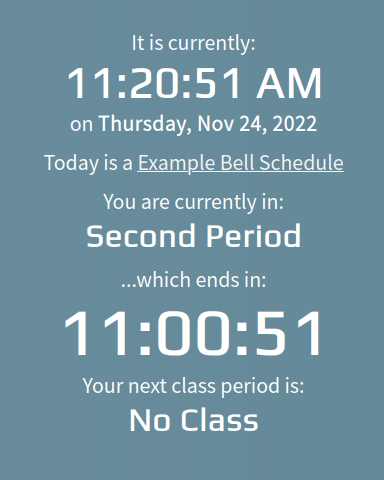
\includegraphics[width=2.1575in,height=2.6972in]{Mini20Manual-img002.png}
{ClassClock began based on an observation that the process for distributing daily bell schedules within a High School
environment was fairly clunky. This included a mixture of techniques from physical printouts of schedules taped to the
wall next to the clock, posts on social media from accounts run by the school or by the student body, or occasional
email announcements and newsletters from the school or district mailing lists. With such a distributed system, it was
hard to pivot quickly when something changed unexpectedly, like an unplanned snow day, \ leaving students constantly
wondering “when will class be over?”}

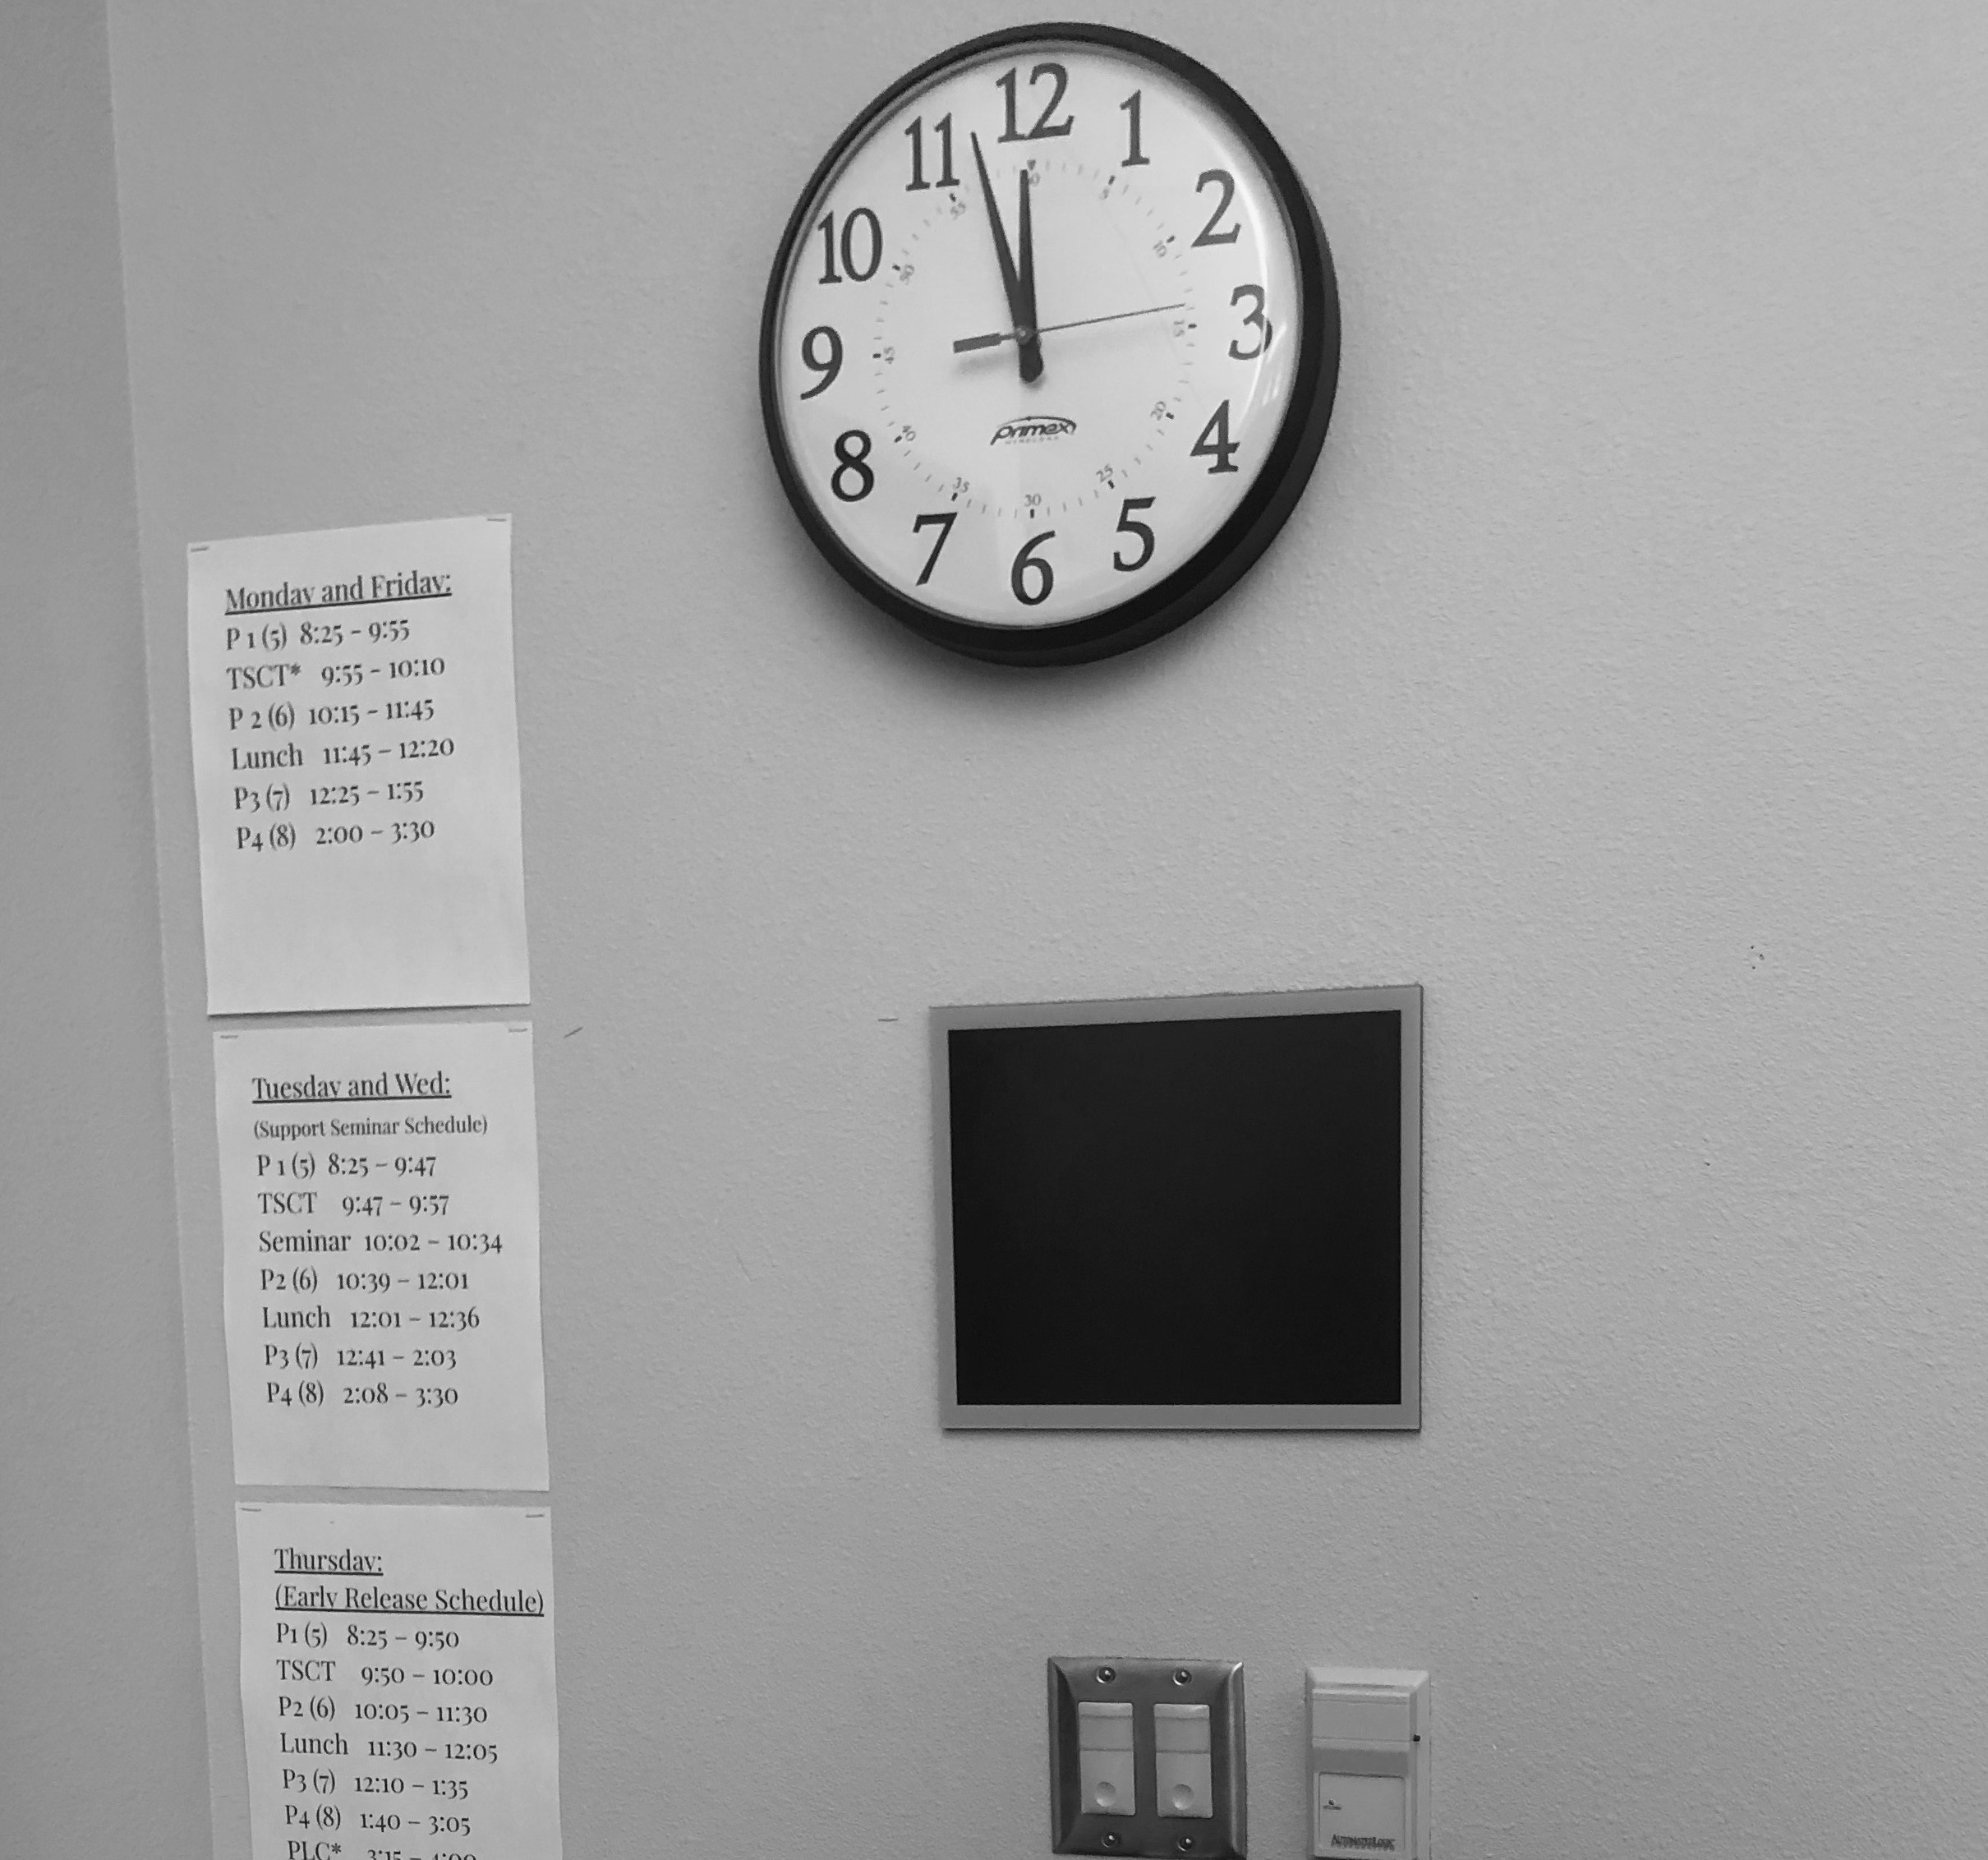
\includegraphics[width=2.9547in,height=2.7646in]{Mini20Manual-img003.jpg}
{ClassClock aims to simplify all of that using common, industry-standard web technologies and ethical software practices
to unify the distribution of school schedule information. The goal is to make it easier for everyone to determine when
class ends by making it easy for schools to distribute schedule information in a consistent, unified way.}

\section{Human Process Description}
{To use the ClassClock software, most users (such as students and school staff) simply need to visit the web address
where ClassClock is located (usually this is https://web.classclock.app) and select their school if they have not
already done so. This makes it quick and easy to access schedule data for users who just need to quickly check that
information and get on with their day. User accounts are not generally needed to simply view schedule data in order to
reduce the barriers and other unnecessary hurdles to accessing information.}

{However, for users who have the ability to modify or delete schedules, a login process is required to ensure that only
users who have been granted permission are able to make changes. This login process protects the administration panel,
which is a frontend that simplifies the process of making changes to schedules.}



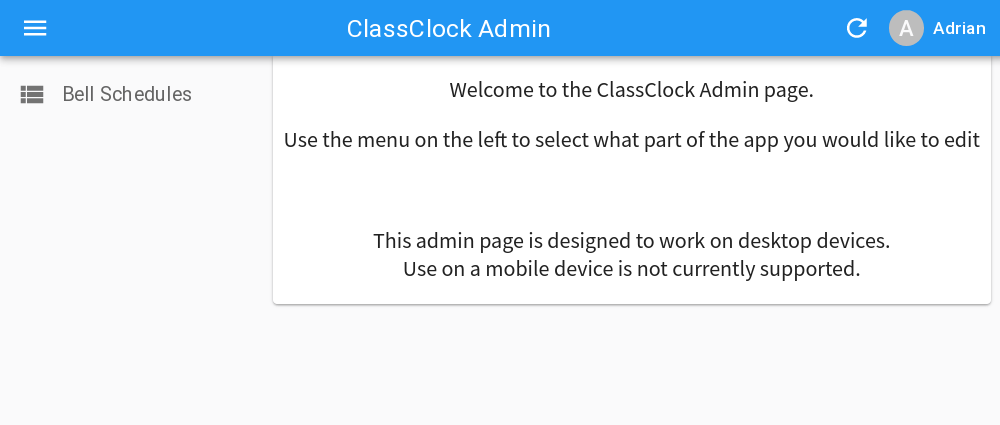
\includegraphics[width=6.5in,height=2.7626in]{Mini20Manual-img004.png}
\section{Objective}
{Given this training manual and access to the ClassClock Admin interface, the trainee will be able to:}

\begin{itemize}
\item {successfully create a new schedule in ClassClock}
\item {successfully assign this new schedule to particular dates}
\item {successfully remove schedules from particular dates}
\end{itemize}
\section{Criterion}
{These tasks should be able to be completed on a reasonably modern desktop/laptop computer and web browser within 10-15
minutes or so.}

{ClassClock is also not intended to be a real-time system and updates may take a while to propagate out to users devices
via the automatic refreshing functionality. It is highly recommended to update schedules at least a day in advance of
when you expect students to use them.}

\section{Target Population Description}
{This training manual is intended for ClassClock users who have some basic experience with the platform and are planning
to maintain ClassClock schedules for their school.}

\subsection{}
\clearpage\section{Training Module}

\bigskip

\setcounter{tocdepth}{9}
\tableofcontents

\bigskip

\subsection{Getting your account set up for the first time}
{The ClassClock admin pages are protected by a login screen. This login screen accepts login with username-and-password
as well as a google account. To get set up with access for the first time:}

\begin{enumerate}
\item {Follow the instructions in the section below to open the admin page}
\item {when you get to the admin page, click on “bell schedules” on the left. This should trigger the login screen to appear if
it didn$\text{\textgreek{’}}$t already. The login screen looks like this:\newline
}
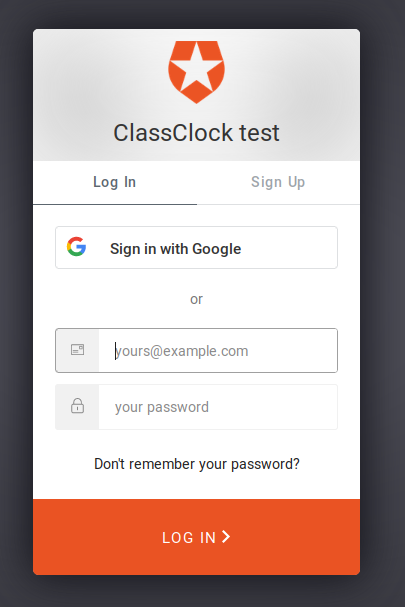
\includegraphics[width=4.2181in,height=6.322in]{Mini20Manual-img005.png}
\item \clearpage{To create your account, select the “Sign up” tab of the login screen and follow the prompts to create your account}
\item {Once your account is created, contact the owner/administrator of your ClassClock server and provide the username and
method you used to sign up (google account or username/password). This is needed in order to assign the appropriate
permissions to your account to give you access to the admin interface. Once this one-time process is done, you should
be able to log in with these credentials to access the admin interface}
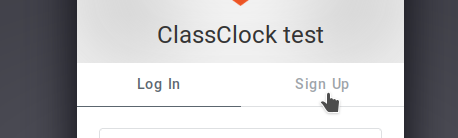
\includegraphics[width=4.7701in,height=1.4366in]{Mini20Manual-img006.png}
\end{enumerate}
\subsection{Opening the ClassClock Admin Page}
\begin{enumerate}
\item {Navigate to the classclock web app in a browser}
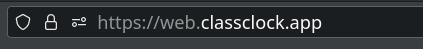
\includegraphics[width=4.4055in,height=0.5102in]{Mini20Manual-img007.png}
\item {If you have not used ClassClock before, select your school. Otherwise, proceed to the next step.}
\item {Go back to the URL bar at the top of the page and type /admin after the URL. This will take you to the admin panel.}
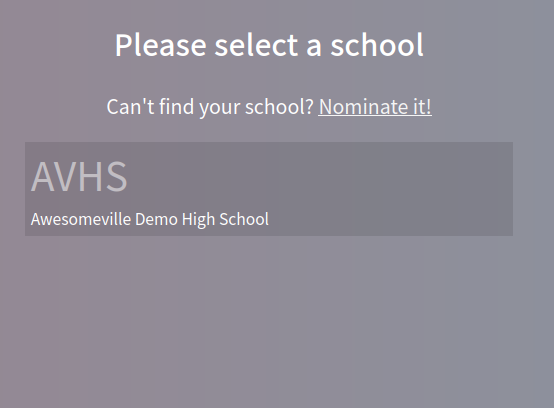
\includegraphics[width=4.0744in,height=1.9016in]{Mini20Manual-img008.png}
\item {You should be provided with a login prompt. If you see this, log in using the credentials (either username and password
or google account login) you used when your school was set up with ClassClock}
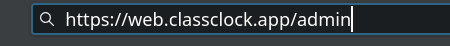
\includegraphics[width=4.6866in,height=0.4783in]{Mini20Manual-img009.png}
\item {You should now see the main admin page (below). From here, click on the “bell schedules” tab. You may be prompted to
sign in}
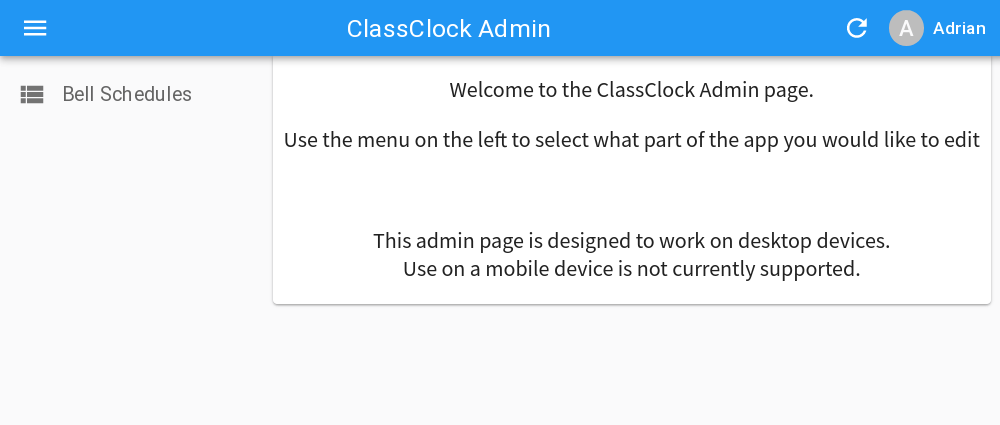
\includegraphics[width=6.5in,height=2.7626in]{Mini20Manual-img004.png}
\end{enumerate}
\subsection{Create a New Bell Schedule}
\begin{enumerate}
\item {To create a new schedule, use the create button in the top right of the calendar.}
\item {Fill out the information for the new schedule, such as in the image below}
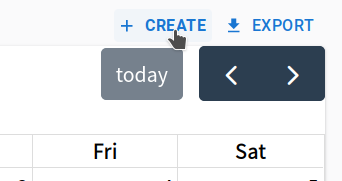
\includegraphics[width=3.8693in,height=1.9382in]{Mini20Manual-img010.png}
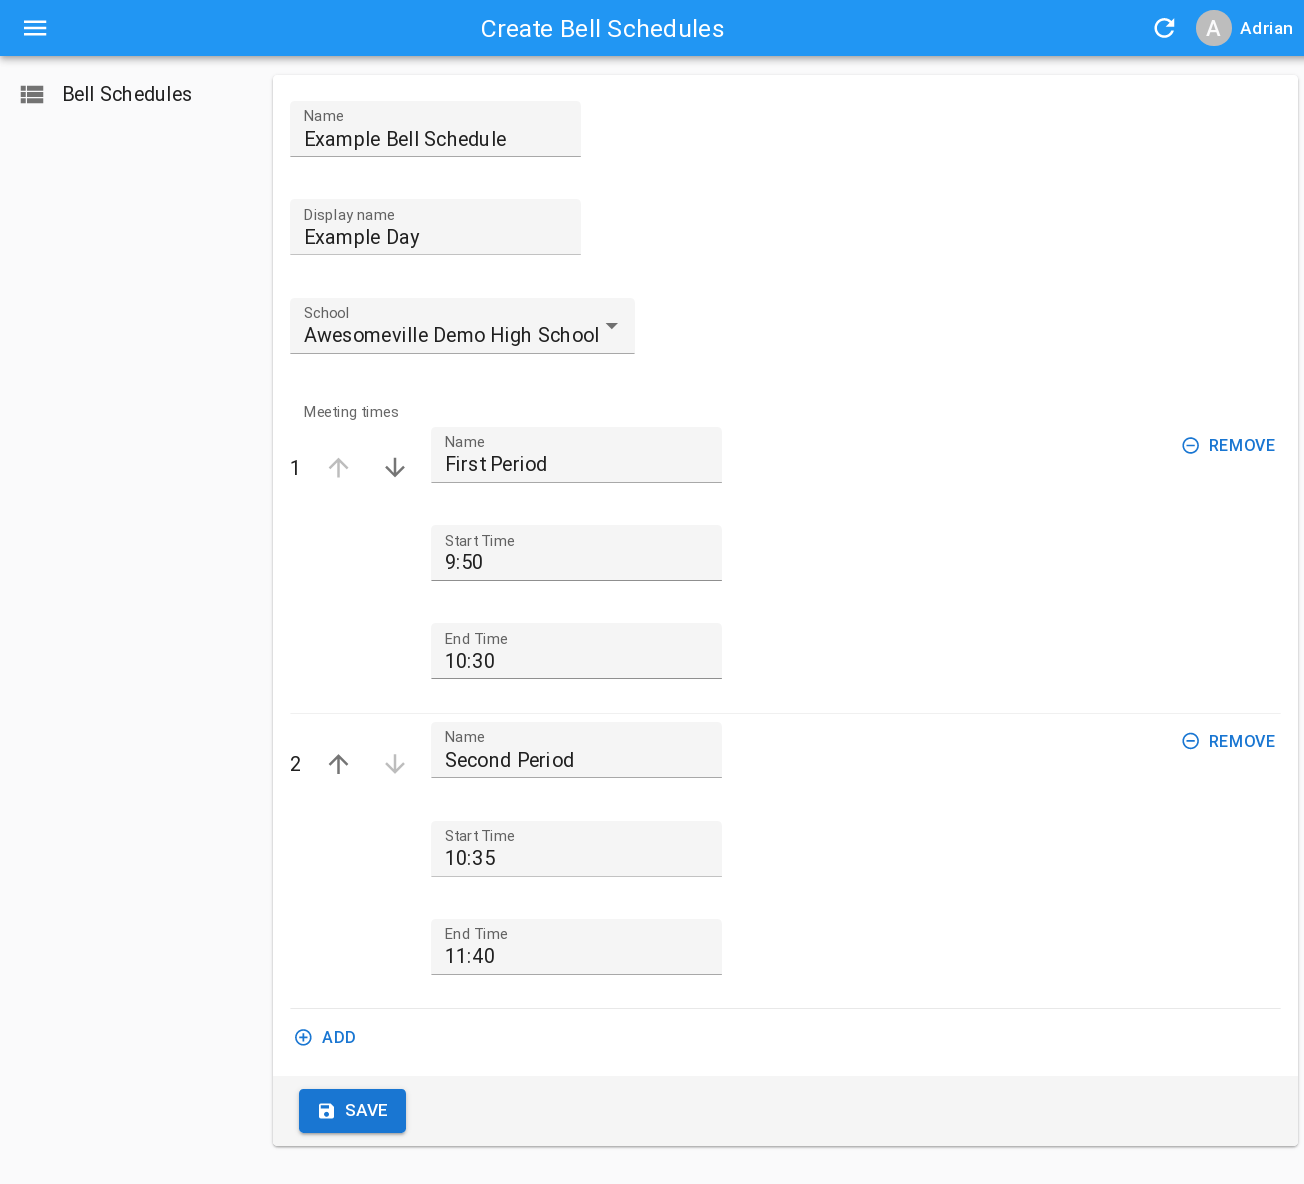
\includegraphics[width=6.5in,height=5.7717in]{Mini20Manual-img011.png}
\item {Click the “Save” Button to save your new schedule}
\end{enumerate}
\clearpage\subsection{Assigning the schedules to Specific days}
\begin{enumerate}
\item {You should see all of your created schedules appear below the calendar. To assign it to a day, click and drag the blue
title of the schedule onto the date that you want to assign it to. You can do this more than once. For this
walkthrough, assign your new schedule to the todays date\newline
}
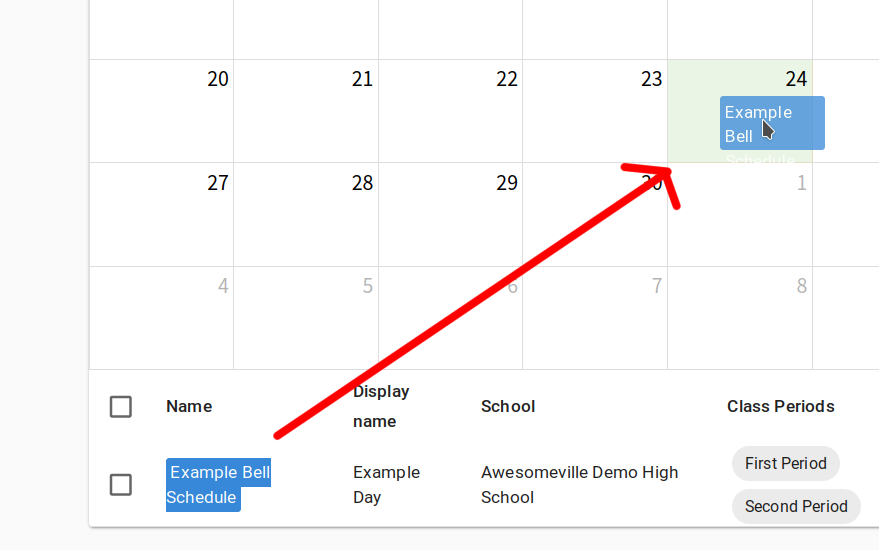
\includegraphics[width=6.5in,height=3.6807in]{Mini20Manual-img012.png}
\item {To verify that your schedule change for the current day worked, open a new tab and navigate back to web.classclock.app.
It will likely still say that you have no school today.}
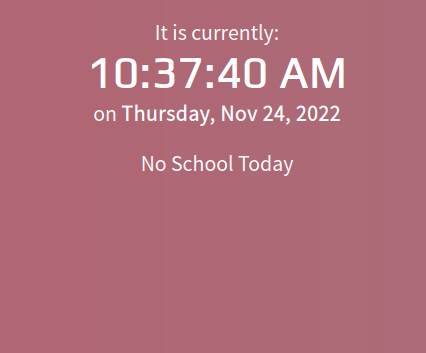
\includegraphics[width=4.4366in,height=2.8764in]{Mini20Manual-img013.png}
\item {\ Click the settings icon in the top left corner}

\includegraphics[width=0.7398in,height=0.7917in]{Mini20Manual-img014.png}
\item {\ Underneath the currently selected school, click the \ “refresh” link }
\item {\ Use the home icon in the top left to navigate back to the main ClassClock page}
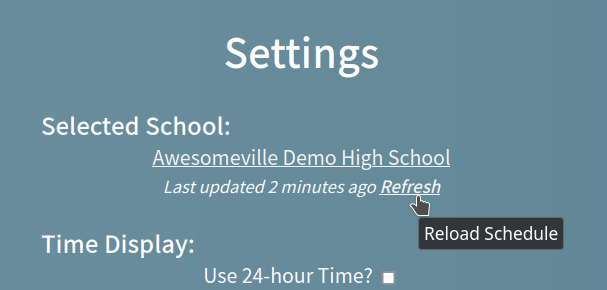
\includegraphics[width=5.511in,height=2.6335in]{Mini20Manual-img015.png}

\includegraphics[width=1.1661in,height=0.8846in]{Mini20Manual-img016.png}
\item \clearpage{Your schedule data should now be populated in the app.}
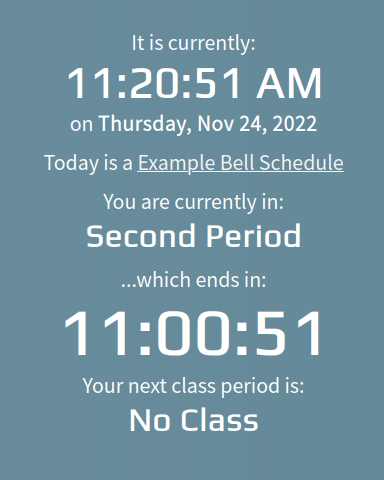
\includegraphics[width=3.9992in,height=4.9992in]{Mini20Manual-img002.png}
\end{enumerate}
\subsection{Duplicating a bell schedule from another day in the calendar}
\begin{enumerate}
\item {All blue items on the admin page are draggable, not just the ones in the table below the calendar. To duplicate a
schedule from another day (such as the same day the previous week), click and drag any existing blue schedule event to
a new empty square on the calendar.\newline
\newline
Be a little patient as duplicating schedules like this is a currently a little slow and takes a second. \newline
\newline
Note each day can only have one schedule assigned to it at a time. If you wish to move a schedule instead of
duplicating, use the method below to remove the original schedule.}
\end{enumerate}
\clearpage\subsection{Removing a bell schedule from a particular day}
\begin{enumerate}
\item {To remove the bell schedule click on the schedule$\text{\textgreek{’}}$s entry in the calendar. It should turn red.
Click again while it is red to remove it.}
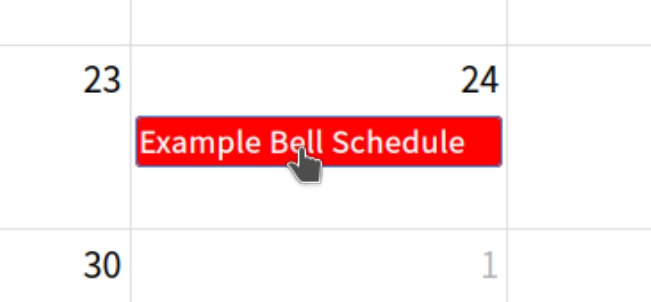
\includegraphics[width=6.5in,height=1.3299in]{Mini20Manual-img017.png}
\item {If you removed the schedule from the current date, refreshing the main ClassClock App should result in the schedule
returning to the “no school today” screen as seen earlier.}
\end{enumerate}
\end{document}
